\documentclass[utf8x, 12pt]{G7-32}

% Настройки стиля ГОСТ 7-32
% Для начала определяем, хотим мы или нет, чтобы рисунки и таблицы нумеровались в пределах раздела, или нам нужна сквозная нумерация.
\EqInChapter % формулы будут нумероваться в пределах раздела
\TableInChapter % таблицы будут нумероваться в пределах раздела
\PicInChapter % рисунки будут нумероваться в пределах раздела
\usepackage{slashbox}

\usepackage[table,xcdraw]{xcolor}

% Добавляем гипертекстовое оглавление в PDF
\usepackage[
bookmarks=true, colorlinks=true, unicode=true,
urlcolor=black,linkcolor=black, anchorcolor=black,
citecolor=black, menucolor=black, filecolor=black,
]{hyperref}

% Изменение начертания шрифта --- после чего выглядит таймсоподобно.
% \usepackage{cyrtimespatched}

% графика
\usepackage{graphicx}
\graphicspath{ {./img/} }

% отделять первую строку раздела абзацным отступом
\usepackage{indentfirst} 

% Пакет Tikz
\usepackage{tikz}
\usetikzlibrary{arrows,positioning,shadows}

% Произвольная нумерация списков.
\usepackage{enumerate}

% ячейки в несколько строчек
\usepackage{multirow}

% itemize внутри tabular
\usepackage{paralist,array}

% объявляем новую команду для переноса строки внутри ячейки таблицы
\newcommand{\specialcell}[2][c]{%
	\begin{tabular}[#1]{@{}c@{}}#2\end{tabular}}

\usepackage{tikz}
\usepackage{pgfplots}
\usepackage{pdfpages}
\usepackage{caption}
\usepackage{longtable}
% \captionsetup[table]{position=top}
% Листинги

\usepackage{listings}
\usepackage{caption}

\usepackage{courier}
\usepackage{wrapfig}

\usepackage{xcolor}
\captionsetup[lstlisting]{singlelinecheck=off, justification=raggedright}


\definecolor{codegreen}{rgb}{0,0.6,0}
\definecolor{codegray}{rgb}{0.5,0.5,0.5}
\definecolor{codepurple}{rgb}{0.58,0,0.82}
\definecolor{backcolour}{rgb}{0.95,0.95,0.92}


% Значения по умолчанию
\lstset{
  % подсветка синтаксиса
  backgroundcolor=\color{backcolour},   
  commentstyle=\color{codegreen},
  keywordstyle=\color{magenta},
  numberstyle=\tiny\color{codegray},
  stringstyle=\color{codepurple},
  basicstyle= \footnotesize,
  breakatwhitespace=true,% разрыв строк только на whitespacce
  breaklines=true,       % переносить длинные строки
%   captionpos=b,          % подписи снизу -- вроде не надо
  inputencoding=koi8-r,
  numbers=left,          % нумерация слева
  numberstyle=\footnotesize,
  showspaces=false,      % показывать пробелы подчеркиваниями -- идиотизм 70-х годов
  showstringspaces=false,
  showtabs=false,        % и табы тоже
  stepnumber=1,
  tabsize=4,              % кому нужны табы по 8 символов?
  frame=single,
  escapeinside={(*}{*)}, %выделение
  literate={а}{{\selectfont\char224}}1
  {б}{{\selectfont\char225}}1
  {в}{{\selectfont\char226}}1
  {г}{{\selectfont\char227}}1
  {д}{{\selectfont\char228}}1
  {е}{{\selectfont\char229}}1
  {ё}{{\"e}}1
  {ж}{{\selectfont\char230}}1
  {з}{{\selectfont\char231}}1
  {и}{{\selectfont\char232}}1
  {й}{{\selectfont\char233}}1
  {к}{{\selectfont\char234}}1
  {л}{{\selectfont\char235}}1
  {м}{{\selectfont\char236}}1
  {н}{{\selectfont\char237}}1
  {о}{{\selectfont\char238}}1
  {п}{{\selectfont\char239}}1
  {р}{{\selectfont\char240}}1
  {с}{{\selectfont\char241}}1
  {т}{{\selectfont\char242}}1
  {у}{{\selectfont\char243}}1
  {ф}{{\selectfont\char244}}1
  {х}{{\selectfont\char245}}1
  {ц}{{\selectfont\char246}}1
  {ч}{{\selectfont\char247}}1
  {ш}{{\selectfont\char248}}1
  {щ}{{\selectfont\char249}}1
  {ъ}{{\selectfont\char250}}1
  {ы}{{\selectfont\char251}}1
  {ь}{{\selectfont\char252}}1
  {э}{{\selectfont\char253}}1
  {ю}{{\selectfont\char254}}1
  {я}{{\selectfont\char255}}1
  {А}{{\selectfont\char192}}1
  {Б}{{\selectfont\char193}}1
  {В}{{\selectfont\char194}}1
  {Г}{{\selectfont\char195}}1
  {Д}{{\selectfont\char196}}1
  {Е}{{\selectfont\char197}}1
  {Ё}{{\"E}}1
  {Ж}{{\selectfont\char198}}1
  {З}{{\selectfont\char199}}1
  {И}{{\selectfont\char200}}1
  {Й}{{\selectfont\char201}}1
  {К}{{\selectfont\char202}}1
  {Л}{{\selectfont\char203}}1
  {М}{{\selectfont\char204}}1
  {Н}{{\selectfont\char205}}1
  {О}{{\selectfont\char206}}1
  {П}{{\selectfont\char207}}1
  {Р}{{\selectfont\char208}}1
  {С}{{\selectfont\char209}}1
  {Т}{{\selectfont\char210}}1
  {У}{{\selectfont\char211}}1
  {Ф}{{\selectfont\char212}}1
  {Х}{{\selectfont\char213}}1
  {Ц}{{\selectfont\char214}}1
  {Ч}{{\selectfont\char215}}1
  {Ш}{{\selectfont\char216}}1
  {Щ}{{\selectfont\char217}}1
  {Ъ}{{\selectfont\char218}}1
  {Ы}{{\selectfont\char219}}1
  {Ь}{{\selectfont\char220}}1
  {Э}{{\selectfont\char221}}1
  {Ю}{{\selectfont\char222}}1
  {Я}{{\selectfont\char223}}1
}

\lstloadlanguages{
  C++
}

% Стиль для псевдокода: строчки обычно короткие, поэтому размер шрифта побольше
\lstdefinestyle{pseudocode}{
  basicstyle=\small,
  keywordstyle=\color{black}\bfseries\underbar,
  language=Pseudocode,
  numberstyle=\footnotesize,
  commentstyle=\footnotesize\it
}

% Стиль для обычного кода: маленький шрифт
\lstdefinestyle{realcode}{
  basicstyle=\scriptsize,
  numberstyle=\footnotesize
}

% Стиль для коротких кусков обычного кода: средний шрифт
\lstdefinestyle{simplecode}{
  basicstyle=\footnotesize,
  numberstyle=\footnotesize
}

% Стиль для BNF
\lstdefinestyle{grammar}{
  basicstyle=\footnotesize,
  numberstyle=\footnotesize,
  stringstyle=\bfseries\ttfamily,
  language=BNF
}

% Определим свой язык для написания псевдокодов на основе Python
\lstdefinelanguage[]{Pseudocode}[]{Python}{
  morekeywords={each,empty,wait,do},% ключевые слова добавлять сюда
  morecomment=[s]{\{}{\}},% комменты {а-ля Pascal} смотрятся нагляднее
  literate=% а сюда добавлять операторы, которые хотите отображать как мат. символы
    {->}{\ensuremath{$\rightarrow$}~}2%
    {<-}{\ensuremath{$\leftarrow$}~}2%
    {:=}{\ensuremath{$\leftarrow$}~}2%
    {<--}{\ensuremath{$\Longleftarrow$}~}2%
}[keywords,comments]

% Свой язык для задания грамматик в BNF
\lstdefinelanguage[]{BNF}[]{}{
  morekeywords={},
  morecomment=[s]{@}{@},
  morestring=[b]",%
  literate=%
    {->}{\ensuremath{$\rightarrow$}~}2%
    {*}{\ensuremath{$^*$}~}2%
    {+}{\ensuremath{$^+$}~}2%
    {|}{\ensuremath{$|$}~}2%
}[keywords,comments,strings]

% Подписи к листингам на русском языке.
\renewcommand\lstlistingname{\cyr\CYRL\cyri\cyrs\cyrt\cyri\cyrn\cyrg}
\renewcommand\lstlistlistingname{\cyr\CYRL\cyri\cyrs\cyrt\cyri\cyrn\cyrg\cyri}



\begin{document}

\frontmatter % выключает нумерацию ВСЕГО; здесь начинаются ненумерованные главы: реферат, введение, глоссарий, сокращения и прочее.
\begin{table}[ht]
	\centering
	\begin{tabular}{|c|p{400pt}|} 
	\hline
		\begin{tabular}[c]{@{}c@{}} 
\includegraphics[scale=0.37]{EmblemBMSTU} \\\end{tabular} &
		\footnotesize\begin{tabular}[c]{@{}c@{}}\textbf{Министерство~науки~и~высшего~образования~Российской~Федерации}\\\textbf{Федеральное~государственное~бюджетное~образовательное~учреждение}\\\textbf{~высшего~образования}\\\textbf{«Московский~государственный~технический~университет}\\\textbf{имени~Н.Э.~Баумана}\\\textbf{(национальный~исследовательский~университет)»}\\\textbf{(МГТУ~им.~Н.Э.~Баумана)}\\\end{tabular}  \\
	\hline
	\end{tabular}
\end{table}
\noindent\rule{\textwidth}{4pt}
\noindent\rule[14pt]{\textwidth}{1pt}
\hfill 
\noindent
\makebox{ФАКУЛЬТЕТ~}%
\makebox[\textwidth][l]{\underline{~~~~«Информатика и системы управления»~~~~~~~~~~~~~~~~~~~~~~~~~~~~~~~~~~~~~~~~~~~~}}%
\\
\noindent
\makebox{КАФЕДРА~}%
\makebox[\textwidth][l]{\underline{~~~~~~~«Программное обеспечение ЭВМ и информационные технологии»~~~~~~~~}}%
\\


\begin{center}
	\vspace{3cm}
	{\bf\huge Отчёт\par}
	{\bf\Large по лабораторной работе №3\par}
	\vspace{0.5cm}
\end{center}


\noindent
\makebox{\large{\bf Название:}~~~}
\makebox[\textwidth][l]{\large\underline{~Алгоритмы сортировок~~~~~~~~~~~~~~~~~~~~~~~~~~~~~~~~~~~~~~~~~~~~~~~~~~~}}\\

\noindent
\makebox{\large{\bf Дисциплина:}~~~}
\makebox[\textwidth][l]{\large\underline{~Анализ алгоритмов~~~~~~~~~~~~~~~~~~~~~~~~~~~~~~~~~~~~~~~~~~~~~~~~~~~~}}\\

\vspace{1.5cm}
\noindent
\begin{tabular}{l c c c c c}
    Студент      & ~ИУ7-55Б~               & \hspace{3.5cm} & \hspace{3.5cm}                 & &  И. Е. Афимин \\\cline{2-2}\cline{4-4} \cline{6-6} 
    \hspace{3cm} & {\footnotesize(Группа)} &                & {\footnotesize(Подпись, дата)} & & {\footnotesize(И.О. Фамилия)}
\end{tabular}

\vspace{1cm}

\noindent
\begin{tabular}{l c c c c}
    Преподаватель & \hspace{6cm}   & \hspace{3.5cm}                 & & Л.Л. Волкова \\\cline{3-3} \cline{5-5} 
    \hspace{3cm}  &                & {\footnotesize(Подпись, дата)} & & {\footnotesize(И.О. Фамилия)}
\end{tabular}

\begin{center}	
	\vfill
	\large \textit {Москва, 2020}
\end{center}

\thispagestyle {empty}
\pagebreak

\tableofcontents

\newpage
\Introduction    
    Алгоритм сортировки -- это алгоритм для упорядочивания элементов в списке.
    Входом является последовательность из n элементов: $ a_1, a_2, \dots, a_n $
    Результатом работы алгоритма сортировки является перестановка
    исходной последовательности $ a'_1, a'_2, \dots, a'_n $,
    такая что $ a_1 \leqslant a_2 \leqslant \dots \leqslant a_n $, 
    где $ \leqslant $ -- отношение порядка на множестве элементов списка.
    Поля, служащие критерием порядка, называются ключом сортировки.
    На практике в качестве ключа часто выступает число,
    а в остальных полях хранятся какие-либо данные, 
    никак не влияющие на работу алгоритма.
    
    В данной работе рассматриваются три алгоритма:
    \begin{enumerate}
        \item сортировка пузырьком с флагом;
        \item сортировка вставками;
        \item сортировка выбором.
    \end{enumerate}

    Целью данной лабораторной работы является реализация алгоритмов сортировки и
    исследование их трудоемкости.

    Задачи данной лабораторной работы:
    \begin{enumerate}
        \item изучить алгоритмы сортировки пузырьком с флагом, вставками, выбором;
        \item реализовать алгоритмы сортировки пузырьком с флагом, вставками, выбором;
        \item дать оценку трудоёмкости в лучшем, произвольном и худшем случае (для двух алгоритмов сделать вывод трудоёмкости);
        \item провести замеры процессорного времени работы для лучшего, худшего и произвольного случая.
    \end{enumerate}

\newpage

\mainmatter % это включает нумерацию глав и секций в документе ниже
\chapter{ Аналитический раздел}
\label{cha:analytical}
    В данном разделе будут рассмотрены основные теоритические понятия алгоритмов сортировок
    пузырьком с флагом, вставками, выбором.

    \section{Алгоритмы сортировок}
	Алгоритм сортировки — это алгоритм для упорядочивания элементов в списке \cite{link3} .
        \subsection{ Алгоритм сортировки пузырьком с флагом}
            Алгоритм сортировки пузырьком или метод простых обменов имеет следующий 
            принцип работы:
            \begin{enumerate}
                \item прохождение по всему массиву;
                \item сравнивание между собой пар соседних ячеек;
                \item если при сравнении оказывается, что значение ячейки i больше, чем значение ячейки i + 1,
                то нужно поменять значения этих ячеек местами.
            \end{enumerate}

            Алгоритм сортировки пузырьком с флагом является модификацией этого алгоритма.
            Идея состоит в том, что если при выполнении прохода методом пузырька не 
            было ни одного обмена элементов массива, то это означает, что массив уже
            отсортирован и остальные проходы не требуются.

        \subsection{ Алгоритм сортировки вставками}
            Алгоритм сортировки вставками, просматривает элементы входной последовательности по одному,
            и для каждого элемента, размещает его в подходящее место среди ранее упорядоченных элементов.
            
            В начальный момент времени отсортированная последовательность пуста. 
            На каждом шаге алгоритма выбирается один из элементов входных данных и
            помещается в нужную позицию в отсортированной последовательности до тех пор,
            пока набор входных данных не будет исчерпан. 
            
            Сортировка методом вставок -- простой алгоритм сортировки. 
            Хотя этот метод сортировки намного менее эффективен,
            чем более сложные алгоритмы (такие как быстрая сортировка), у него есть ряд преимуществ
            \begin{enumerate}
                \item простота реализации;
                \item эффективен на небольших наборах данных;
                \item эффективен на частично отсортированных последовательностях;
                \item является устойчивым алгоритмом (не меняет порядок элементов, которые уже отсортированы).
            \end{enumerate}

        \subsection{ Алгоритм сортировки выбором}
            Алгоритм сортировки выбором работает следующим образом: 
            находим наименьший элемент в массиве и обмениваем его с элементом находящимся на первом месте.
            Повторяем процесс -- находим наименьший элемент в последовательности, начиная со второго элемента, и
            обмениваем со вторым элементном и так далее, пока весь массив не будет отсортирован.
            Этот метод называется сортировка выбором, поскольку он работает, 
            циклически выбирая наименьший из оставшихся элементов.

            Главным отличием сортировки выбором от сортировки вставками является, то что в сортировке вставками 
            извлекается из неотсортированной части массива первый элемент (не обязательно минимальный) и
            вставляется на своё место в отсортированной части.
            В отличии от сортировки выбором, где ищется минимальный элемент 
            в неотсортированной части,  который вставляется в конец отсортированной части массива.

\section{Вывод}
Были рассмотрены алгоритмы сортировки пузырьком, вставками и выбором. Каждый имеет свою особенность, а конкретно сложность работы в лучшем/худшем случаях.




\chapter{Конструкторская часть}
    В данном разделе будут рассмотрены требования к функциональности ПО, схемы алгоритмов
    и определены способы тестирования.

    \section{Требования к функциональности ПО}
        В данной работе требуется обеспечить следующую минимальную функциональность консольного приложения.
            \begin{enumerate}
                \item возможность подать на вход массив;
                \item при массиве нулевой длины программа не должна аварийно завершаться;
		\item корректная сортировка;
	      \item обеспечить вывод замеров времени работы каждого из алгоритмов в худшем, лучшем и произвольном случаях.
            \end{enumerate}
\section{Тесты}
    Тестирование ПО будет проводиться методом чёрного ящика. Необходимо проверить работу системы 
    на массивах различных длин.

    \section{Схемы алгоритмов}
        Ниже будут представлены схемы алгоритмов нахождениея произведения матриц: \begin{enumerate}
            \item Схема сортировки пузырьком (рисунок \ref{schema:num_1});
            \item Схема сортировки вставками (рисунок \ref{schema:num_2});
            \item Схема сортировки выбором (рисунок \ref{schema:num_3});
        \end{enumerate}

    \begin{figure}[!htbp]
        \centering
        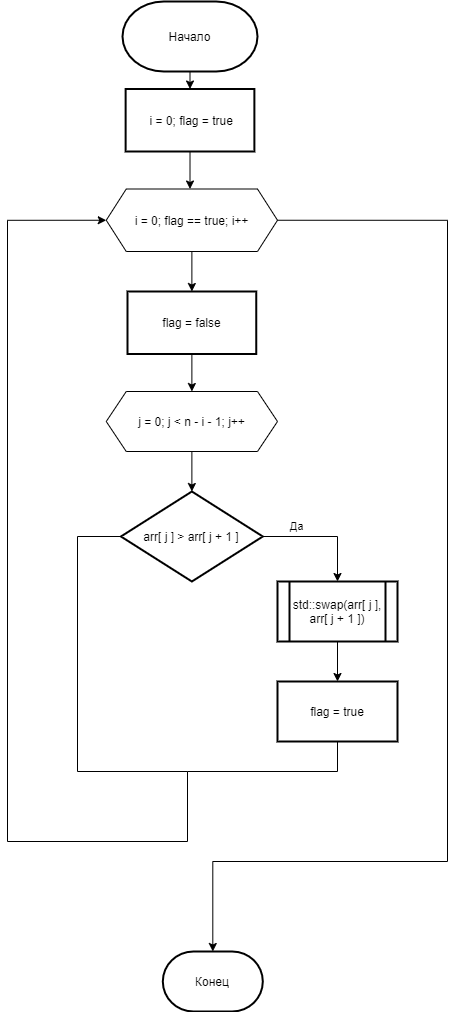
\includegraphics[scale=0.6]{Bubble}
        \caption{Схема сортировки пузырьком}
        \label{schema:num_1}
    \end{figure}

    \begin{figure}[!htbp]
        \centering
        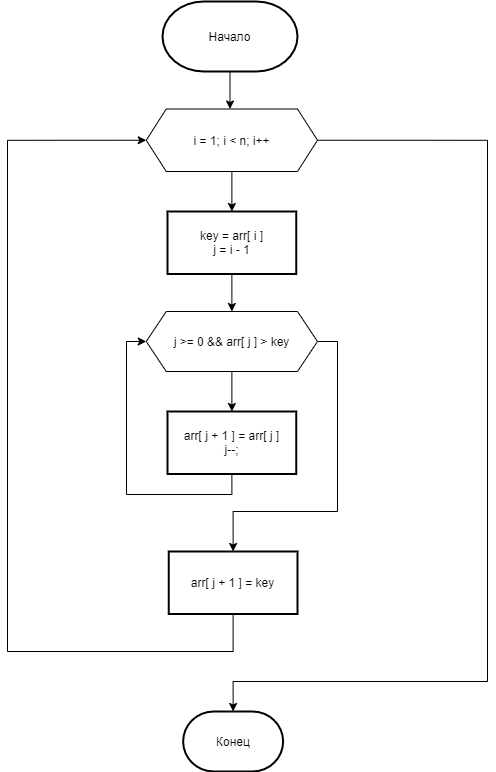
\includegraphics[scale=0.63]{Insertion}
        \caption{Схема сортировки вставками}
        \label{schema:num_2}
    \end{figure}

    \begin{figure}[!htbp]
        \centering
        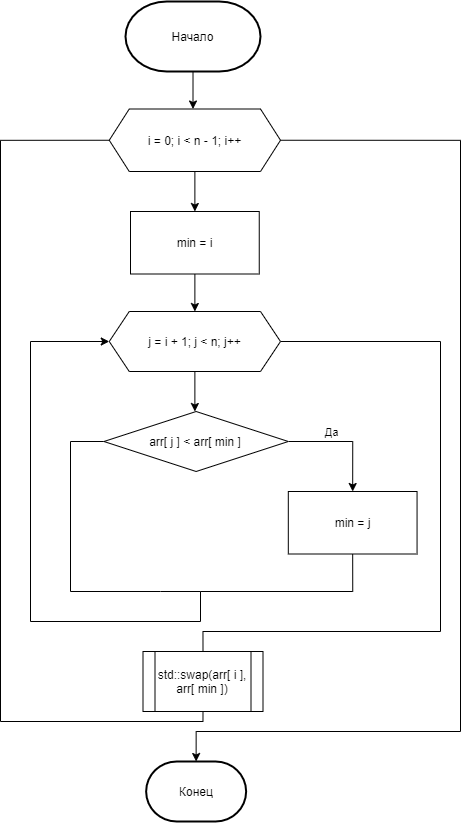
\includegraphics[scale=0.8]{Quick}
        \caption{Схема сортировки выбором}
        \label{schema:num_3}
    \end{figure}

\newpage
 \section{Трудоёмкость алгоритма}
        Трудоёмкость -- количество работы, которую алгоритм затрачивает на обработку данных.
        Является функцией от длины входов алгоритма и позволяет оценить количество работы.

        Введём модель вычисления трудоёмкости.

        \subsection{Базовые операции}
            Ниже представлены базовые операции, стоимость которых единична:
            \begin{enumerate}
                \item $ =, +, +=, -, -=, *, *=,  /, /=, ++, --, \% $,
                \item $ <, \leqslant, ==, \neq, \geqslant , > $,
                \item $ [ $  $ ] $.
            \end{enumerate}
            
        \subsection{Условный оператор}
            if (условие) \{

                // тело A

            \}

            else \{

                // тело B
            
            \}

            Пусть трудоёмкость тела A равна $ f_A $, а тела B $ f_B $, тогда
            стоимость условного оператора можно найти по формуле (\ref{equation:trud:if}):
            \begin{equation}
                f_{if} = f_\text{условия} + \left\{
                    \begin{matrix}
                    min(f_A, f_B) - \text{лучший случай},\\
                    max(f_A, f_B) - \text{худший случай} 
                    \end{matrix}\right.
                \label{equation:trud:if}
            \end{equation}

        \subsection{Цикл со счётчиком}
            for (int i = 0; i < n; i++) \{

                // тело цикла

            \}
            
            Начальная инициализация цикла (int i = 0) выполняется один раз.
            Условие i < n проверяется перед каждой итерацией цикла и при входе в цикл -- n + 1 операций.
            Тело цикла выполняется ровно n раз.
            Счётчик (i++) выполняется на каждой итерации, перед проверкой условия, т.е. n раз.
            Тогда, если трудоёмкость тела цикла равна $ f $, трудоёмкость всего цикла определяется формулой (\ref{equation:trud:for})

            \begin{equation}
                f_\text{цикла} = 2 + n(2 + f)
                \label{equation:trud:for}
            \end{equation}

\newpage
\subsection{Алгоритм сортировки пузырьком с флагом}
 
\textbf{Лучший случай:} Массив отсортирован; не произошло ни одного обмена за 1 проход -> выходим из цикла \newline
Трудоемкость:
            \begin{equation}
                f = 1 + 2 + (2 + 1 + 2 + (N - 1) (2 + 3) + 2) = 5N + 8= O(N)
            \end{equation}
\textbf{Худший случай:}  Массив отсортирован в обратном порядке; в каждом случае происходил обмен\newline
Трудоемкость: 
 	\begin{equation}
                f = 1 + 2 + \sum_{i=1}^N (2 + 1 + 2 + (N - i)(2 + 4) + 1) = 3N^2 + 3N + 3 = O(N^2)
            \end{equation}


\subsection{Алгоритм сортировки вставками}
\hspace*{5mm}
\textbf{Лучший случай:} отсортированный массив. При этом все внутренние циклы состоят всего из одной итерации.\newline
Трудоемкость:
	\begin{equation}
                f = 1 + 2 + (N-1)(2 + 3 + 2 + 2 + 1) = 10N - 7 = O 
            \end{equation}

\textbf{Худший случай:} массив отсортирован в обратном нужному порядке. Каждый новый элемент сравнивается со всеми в отсортированной последовательности.
Все внутренние циклы будут состоять из j итераций. \newline
Трудоемкость: 
            \begin{equation}
                f = 1 + 2 + (N-1)(2 + 3 + \sum_{i=1}^{N-1} (2 + 2 + 1 + 4 + 1) + 1) = 10N^2 - 14N + 7 = O(N^2)
            \end{equation}

\subsection{Алгоритм сортировки выбором}
            Трудоёмкость сортировки выбором в худшем и лучшем случаях совпадает
            и оценивается как $ O(N^2) $.

\section{Вывод}
Сортировка пузырьком: лучший - $O(n)$, худший - $O(n^2)$ \newline
Сортировка вставками: лучший - $O(n)$, худший - $O(n^2)$ \newline
Сортровка выбором: лучший - $O(n^2)$, худший - $O(n^2)$ \newline




\chapter{Технологическая часть}
В данном разделе будут выбраны средства реплизации ПО, представлен листинг кода
и будет показан метод тестирования.
\section{Средства реализации}
Для реализации программ я выбрал язык программирования C++, так как имею большой опыт работы с ним.
Для замера процессорного времени была использована ассемблерная вставка \cite{link_time}.


\section{Сведения о модулях программы}
Программа состоит из:
\begin{itemize}
	\item main.cpp - главный файл программы, в котором располагается точка входа в программу.
	\item main\_test.cpp - файл с функциями тестирования и замера времени.
	\item sort\_algorithms.cs - файл c реализациями 3-х алгоритмов сортировки.
\end{itemize}

    \section{Листинг программы}
        Ниже представлены листинги кода поиска растояния Левенштейна: \begin{enumerate}
            \item сортировка пузырьком (листинг \ref{num_1});
            \item сортировка вставками (листинг \ref{num_2});
            \item сортировка выбором (листинг \ref{num_3}).
        \end{enumerate}

\begin{lstlisting}[label=num_1,caption=Сортировка "Пузырьком", escapechar=@]
void Bubble_Sort(IArr_t arr, int n)
{
    int i = 0;
    bool flag = true;

    while (flag)
    {
        flag = false;
        for (int j = 0; j < n - i - 1; j++)
        {
            if (arr[j] > arr[j + 1])
            {
                std::swap(arr[j], arr[j + 1]);
                flag = true;
            }
        }

        i++;
    }
}
\end{lstlisting}


\begin{lstlisting}[label=num_2,caption=Сортировка вставками]
void InserionSort(IArr_t arr, int n)
{
    int key, j;
    for (int i = 1; i < n; i++)
    {
        key = arr[i];
        j = i - 1;

        while (j >= 0 && arr[j] > key)
        {
            arr[j + 1] = arr[j];
            j--;
        }

        arr[j + 1] = key;
    }
}
\end{lstlisting}


\begin{lstlisting}[label=num_3,caption=Сортировка выбором, escapechar=@]
void Selection_Sort(IArr_t arr, int n)
{
    for (int i = 0; i < n - 1; i++)
    {
        int min = i;
        for (int j = i + 1; j < n; j++)
        {
            if (arr[j] < arr[min])
            {
                min = j;
            }
        }

        std::swap(arr[i], arr[min]);
    }
}
\end{lstlisting}

\section{Тестирование}
В таблице \ref{table:testing} отображён возможный набор тестов для тестирования методом чёрного ящика.
В столбцах Пузырёк,  Вставки,  Выбором представлены соответсвенно результаты сортировки массива, полученные алгоритмом сортировки пузырьком, алгоритмом сортировки вставками и выбором.


\begin{table}[]
            \caption{Таблица тестовых данных}
	    \centering
            \begin{tabular}{|c|c|c|c|c|}
            \hline
            № & Массив & \begin{tabular}[c]{@{}c@{}}Пузырёк\\\end{tabular} & \begin{tabular}[c]{@{}c@{}}Вставки\\ \end{tabular} & \begin{tabular}[c]{@{}c@{}}Выбором\\ \end{tabular} \\ \hline
 	1 & 1 2 3 4  & 1 2 3 4 & 1 2 3 4 & 1 2 3 4\\
	\hline
	2 & 1 4 3 2 & 1 2 3 4 & 1 2 3 4 & 1 2 3 4 \\
	\hline
	3 &  4 3 2 1 & 1 2 3 4 & 1 2 3 4 & 1 2 3 4\\
	\hline
	4 & 5 & 5 & 5 &  5\\
	\hline
            \end{tabular}
            \label{table:testing}
\end{table}

\section{Вывод}
В данном разделе были представлены реализации алгоритмов сортировки пузырьком, вставками и выбором. А также представлен, успешно пройденный, набор тестов.


\chapter{Экспериментальный раздел}
\label{cha:research}
    В данном разделе будут проведены эксперименты для проведения 
    сравнительного анализа трёх алгоритмов по затрачиваемому процессорному 
    времени в зависимости от длины массива и степени его отсортированности.

    \section{Сравнительный анализ на основе замеров времени работы алгоритмов}
        В рамках данного проекта были проведёны следующие эксперименты:
        \begin{enumerate}
            \item сравнение времени работы алгоритмов в лучшем случае (графики \ref{graph:test:best}, \ref{graph:test:best1});
            \item сравнение времени работы алгоритмов в худшем случае (график \ref{graph:test:bad});
            \item сравнение времени работы алгоритмов в произвольном случае (график \ref{graph:test:random}).
        \end{enumerate}

	Для построения графиков 
        указанные массивы генерировались размерами от 1 до 10000.

        Тестирование проводилось на ноутбуке с процессором
        Intel(R) Core(TM) i5-8250U CPU 1.60 GHz
        под управлением Windows 10 с 8 Гб оперативной памяти.


    \begin{figure}[h!]
        \centering
        \begin{tikzpicture}
            \begin{axis}[
                legend pos = north west,
                grid = major,
                xlabel = Размер массива,
                ylabel = {Время, сек},
                height = 0.5\paperheight, 
                width = 0.75\paperwidth
            ]
            
            \addplot table[x=n,y=bubble] {data/test-best.dat};
            \addplot table[x=n,y=insertion] {data/test-best.dat};
            \addplot table[x=n,y=selection] {data/test-best.dat};
            \legend{
                Сортировка пузырьком,
                Сортировка вставками,
                Сортировка выбором,
            };
            \end{axis}
        \end{tikzpicture}
        \caption{График зависимости времени работы реализации алгоритмов сортировки в лучшем случае} 
        \label{graph:test:best}
    \end{figure}

    \begin{figure}[h!]
        \centering
        \begin{tikzpicture}
            \begin{axis}[
                legend pos = north west,
                grid = major,
                xlabel = Размер массива,
                ylabel = {Время, сек},
                height = 0.5\paperheight, 
                width = 0.75\paperwidth
            ]
            
            \addplot table[x=n,y=bubble] {data/test-best.dat};
            \addplot table[x=n,y=insertion] {data/test-best.dat};
            \legend{
                Сортировка пузырьком,
                Сортировка вставками,
                Сортировка выбором,
            };
            \end{axis}
        \end{tikzpicture}
        \caption{График зависимости времени работы реализации алгоритмов сортировки пузырьком и вставками в лучшем случае} 
        \label{graph:test:best1}
    \end{figure}

    \begin{figure}[h!]
        \centering
        \begin{tikzpicture}
            \begin{axis}[
                legend pos = north west,
                grid = major,
                xlabel = Размер массива,
                ylabel = {Время, сек},
                height = 0.5\paperheight, 
                width = 0.75\paperwidth
            ]
            
            \addplot table[x=n,y=bubble] {data/test-bad.dat};
            \addplot table[x=n,y=insertion] {data/test-bad.dat};
            \addplot table[x=n,y=selection] {data/test-bad.dat};
            \legend{
                Сортировка пузырьком,
                Сортировка вставками,
                Сортировка выбором,
            };
            \end{axis}
        \end{tikzpicture}
        \caption{График зависимости времени работы реализации алгоритмов сортировки в худшем случае} 
        \label{graph:test:bad}
    \end{figure}

    \begin{figure}[h!]
        \centering
        \begin{tikzpicture}
            \begin{axis}[
                legend pos = north west,
                grid = major,
                xlabel = Размер массива,
                ylabel = {Время, сек},
                height = 0.5\paperheight, 
                width = 0.75\paperwidth
            ]
            
            \addplot table[x=n,y=bubble] {data/test-random.dat};
            \addplot table[x=n,y=insertion] {data/test-random.dat};
            \addplot table[x=n,y=selection] {data/test-random.dat};
            \legend{
                Сортировка пузырьком,
                Сортировка вставками,
                Сортировка выбором,
            };
            \end{axis}
        \end{tikzpicture}
        \caption{График зависимости времени работы реализации алгоритмов сортировки в произвольном случае} 
        \label{graph:test:random}
    \end{figure}

\newpage


\section{Вывод}
 В ходе экспериментов по замеру времени работы было установлено, что 
        в лучшем случае, когда массив отсортирован, сортировка выбором оказалась самой медленной.
        Алгоритм сортировки вставками оказался медленнее сортировки вставками.
        Сортировка пузырьком с флагом в лучшем случае работает быстрее всего.

        В худшем случае самой медленной сортировкой является сортировка пузырьком с флагом,
        а сортировка выбором является самой быстрой (более, чем в 2 раза быстрее сортировки с флагом).

        В произвольном случае время работы сортировок вставками и выбором сопоставимо.
        Самой медленной является сортировка пузырьком с флагом.


\Conclusion
    В ходе работы были изучены и реализованы алгоритмы сортировки
    (пузырьком с флагом, вставки и выбором). А также дана оценка их трудоемкости и замерено процессорное время работы алгоритмов.
    
    В ходе экспериментов по замеру времени работы было установлено, что 
    в лучшем случае, когда массив отсортирован, сортировка выбором оказалась самой медленной.
    Алгоритм сортировки вставками оказался быстрее сортировки выбором.
    Сортировка пузырьком с флагом в лучшем случае работает быстрее всего.

    В худшем случае самой медленной сортировкой является сортировка пузырьком с флагом,
    а сортировка выбором является самой быстрой (более, чем в 2 раза быстрее сортировки с флагом).

    В произвольном случае время работы сортировок вставками и выбором сопоставимо.
    Самой медленной является сортировка пузырьком с флагом.
 
%далее сам список используевой литературы
\begin{thebibliography}{}
    \bibitem{link_time}  Ассемблерные вставки в AVR-GCC. // [Электронный ресурс]. Режим доступа: http://we.easyelectronics.ru/AVR/assemblernye-vstavki-v-avr-gcc.html, (дата обращения: 15.10.2020).
    \bibitem{link2}  C/C++: как измерять процессорное время. // [Электронный ресурс]. Режим доступа: https://habr.com/ru/post/282301/, (дата обращения: 15.10.2020).
    \bibitem{link3}  Sorting algorithm. // [Электронный ресурс]. Режим доступа: $https://en.wikipedia.org/wiki/Sorting_algorithm$, (дата обращения: 15.10.2020).
\end{thebibliography}

\end{document}